\documentclass[12pt]{extarticle}
\usepackage[utf8]{inputenc}
\usepackage[margin =0.5in]{geometry}
\usepackage[inline]{enumitem}  
\usepackage{tabularx}
\usepackage{amsmath}
\usepackage{graphicx}
\graphicspath{ {./images/} }


\author{Sean Balbale}
\date{September 2022}

\begin{document}
\section*{AP Chemistry: Chapter 8 Summary}
\begin{enumerate*}[label={}]
    \item Name: Sean Balbale
    \item September, 2022
\end{enumerate*}
\subsection*{8.1: Types of Chemical Bonds}
The energy interaction between a pair of ions can be calculated using Coulomb's law
\\$E=(2.31 \times 10^{-19} J \cdot nm)\cdot(\frac{Q_1Q_2}{r})$
\\\textbf{Variables:}
\begin{itemize}[label={}]
    \item $E$: Energy, Joules
    \item $r$: Distance between ion centers, Nanometers
    \item $Q_1$, $Q_2$: numerical ion charges
\end{itemize}
\textbf{Covalent Bonding:}
The type of bonding in which electrons are shared by nuclei.
\\\textbf{Ionic Bonding:}
The type of bonding from electrostatic attraction between oppositely charged ions.
\\\textbf{Bond Length:}
The distance where the attractive and retractive forces result in an energy minimum

\subsection*{8.2: Electronegativity}
\textbf{Electronegativity:}
The ability of an atom in a molecule to attract shared electrons to itself.
\\\textbf{How to calculate values of electronegativity:}
$\text{Expected }H - X_{\text{bond energy}} = \frac{H-H_{\text{bond energy}} + X- X_{\text{bond energy}}}{2}$
\\The difference between actual and expected bond energies is:
$\Delta = (H-X)_{act} - (H-X)_{exp}$
\\ If H and X have identical electronegativities then $(H-X)_{act}$ and $(H-X)_{exp}$ will be the same and $\Delta$ is 0.
\\ Otherwise if X or H has a greater electronegativity than the shared electron(s) will be closer to that atom.
\\ The molecule will be polar and have the following charge distribution: $\underset{\delta^+\delta^-}{H-X}$

\subsection*{8.3: Bond Polarity and Dipole Moments}
\textbf{Dipole moment:}
a property of a molecule whose charge distribution can be represented by a center of positive charge and a center of negative charge.
\\\textbf{Dipolar: }
A molecule that has a center of positive charge and a center of negative charge, to have a dipole moment
\\ The dipolar character of a molecule is often represented by an arrow pointing to the negative charge center with the tail of the arrow indicating the positive center of charge
\begin{center}
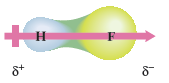
\includegraphics[scale=0.75]{DipolarEX.png}
\end{center}

\subsection*{8.4: Ions: Electron Configurations and Sizes}
\begin{itemize}
    \item {When \textit{two nonmetals} react to form a covalent bond, they share electrons in a way that completes the valence electron configurations of both atoms. That is, both nonmetals attain noble gas electron configurations.}
    \item{ When a \textit{nonmetal and a representative-group meta}l react to form a binary ionic compound, the ions form so that the valence electron configuration of the nonmetal achieves the electron configuration of the next noble gas atom and the valence orbitals of the metal are emptied. In this way both ions achieve noble gas electron configurations.}
\end{itemize}
\subsubsection*{Predicting Formulas of Ionic Compounds}
To predict the formula of an ionic compound we can use the fact that chemical compounds are always electrically neutral and the emperical formula.
\subsubsection*{Sizes of Ions}
\textbf{Isoelectronic ions:}
ions containing the same number of electrons.
\\There are many factors that influence ion size, we will only look at trends.
\\Ion sizes increase as you move down the periodic table.
\subsection*{8.5: Energy Effects in Binary Ionic Compounds}
\textbf{Lattice Energy:}
The change in energy that takes place when separated gaseous ions are packed together to form an ionic solid.
\\$M^+(g) + X^-(g) \rightarrow MX(s)$
\\The lattice energy is often defined as the energy \textit{released} when an ionic solid forms from its ions.
\\The lattice energy has a negative sign (-)
\subsubsection*{Lattice Energy Calculations}
Lattice energy can be represented by a modified form of Coulomb’s law:
\\$\text{Lattice energy} = k(\frac{Q_1Q_2}{r})$
\\\textbf{Variables:}
\begin{itemize}[label={}]
    \item $k$: Proportionality constant that depends on the structure and electron configuration
    \item $r$: Distance between ion centers, Nanometers
    \item $Q_1$, $Q_2$: numerical ion charges
\end{itemize}

\subsection*{8.6: Partial Ionic Character of Covalent Bonds}
There are no totally ionic bonds between discrete pairs of atoms
\\\textbf{Percent ionic character of a bond:}
\\$\text{Percent ionic character of a bond} = (\frac{\text{measured dipole moment of X-Y}}{\text{calculated dipole moment of X$^+$Y$^-$}})\times100\%$
\\Any compound that conducts an electric current when melted will be classified as ionic.

\subsection*{8.7: The Covalent Chemical Bond: A Model}
\textbf{What is a chemical bond:}
Chemical bonds can be viewed as forces that cause a group of atoms to behave as a unit.
\\\textbf{Why do chemical bonds occur:}
Bonds result from the tendency of a system to seek its lowest possible energy.
\subsubsection*{Models: An Overview}
\begin{itemize}
    \item Models are human inventions, always based on an incomplete understanding of how nature works. A model does not equal reality.
    \item Models are often wrong. This property derives from the first property. Models are based on speculation and are always oversimplifications.
    \item Models tend to become more complicated as they age. As flaws are discovered in our models, we “patch” them and thus add more detail.
    \item For a model to be used effectively, we must understand its strengths and weaknesses
    \item When a model is wrong, we often learn much more than when it is right. If a model makes a wrong prediction, it usually means we do not understand some fundamental characteristics of nature. 
\end{itemize}

\subsection*{8.8: Covalent Bond Energies and Chemical Reactions}
\textbf{Single Bond:}
The bond that is formed when atoms share one electron.
\\\textbf{Double Bond:}
The bond that is formed when atoms share two electrons.
\\\textbf{Triple Bond:}
The bond that is formed when atoms share three electrons.
\subsubsection{Bond Energy and Enthalpy}
Bond energy values can be used to calculate approximate energies for reactions.
\\$\Delta H = $ sum of the energies required to break old bonds (positive) plus the sum of the energies released in the formation of the new bonds (negative)
\\$\Delta H = \Sigma n \times D \text{(bonds broken)} - \Sigma n \times D \text{(bonds formed)}$
\\\textbf{Variables:}
\begin{itemize}[label={}]
    \item $\Sigma$: Sum of terms
    \item $D$: Bond energy per mole of bonds (always positive)
    \item $n$: Moles of a particular type of bond
\end{itemize}

\subsection*{8.9: The Localized Electron Model}
\textbf{Localized Electron (LE) Model Assumes:}
a molecule is composed of atoms that are bound together by sharing pairs of electrons using the atomic orbitals of the bound atoms.
\\\textbf{Lone Pairs:}
Pairs of electrons localized on an atom
\\\textbf{Bonding Pairs:}
Pairs of electrons found in the space between atoms.
\\The LE Model has three parts:
\begin{enumerate}
    \item Description of the valence electron arrangement in the molecule using Lewis structures
    \item Prediction of the geometry of the molecule using the valence shell electron-pair repulsion (VSEPR) model
    \item Description of the type of atomic orbitals used by the atoms to share electrons or hold lone pairs
\end{enumerate}

\subsection*{8.10: Lewis Structures}
The Lewis structure of a molecule shows how the valence electrons are arranged.
\\The most important requirement for the formation of a stable compound is that the atoms achieve noble gas electron configurations.
\\\textbf{Duet Rule:}
Hydrogen and Helium form stable molecules when it shares two electrons.
\\\textbf{Octet Rule:}
The observation that atoms of nonmetals tend to form the most stable molecules when they are surrounded by eight electrons
\newpage
\textbf{Steps for Writing Lewis Structures}
\begin{enumerate}
    \item Sum the valence electrons from all the atoms.
    \item Use a pair of electrons to form a bond between each pair of bound atoms.
    \item Arrange the remaining electrons to satisfy the duet rule for hydrogen and the octet rule for the second-row elements.
\end{enumerate}

\subsection*{8.11: Exceptions to the Octet Rule}
\begin{enumerate}
    \item C,N,O,F should always be assumed to obey the octet rule.
    \item B and Be often have fewer than eight electrons around them in compounds. These electron-deficient compounds are very reactive.
    \item The second-row elements never exceed the octet rule, since their valence orbitals (2s and 2p) can accommodate only eight electrons.
    \item Third-row and heavier elements often satisfy the octet rule but can exceed the octet rule by using their empty valence d orbitals.
    \item When writing the Lewis structure for a molecule, satisfy the octet rule for the atoms first. If electrons remain after the octet rule has been satisfied, then place them on the elements having available d orbitals
\end{enumerate}

\subsection*{8.12: Resonance}
Sometimes more than one valid Lewis structure (one that obeys the rules we have outlined) is possible for a given molecule.
We can solve this problem by making the following assumption: The correct description is not given by any one of the three Lewis structures but is given only by the superposition of all three.
\textbf{Resonance: }
a condition occurring when more than one valid Lewis structure can be written for a particular molecule. The actual electronic structure is not represented by any one of the Lewis structures but by the average of all of them.
\subsubsection*{Odd-Electron Molecules}
Relatively few molecules formed from nonmetals contain odd numbers of electrons. Since the localized electron model is based on pairs of electrons, it does not handle odd-electron cases in a natural way. To treat odd-electron molecules, a more sophisticated model is needed.
\subsubsection*{Formal Charge}
\textbf{Formal Charge:}
The charge assigned to an atom in a molecule or polyatomic ion derived from a specific set of rules.
\\The formal charge of an atom in a molecule is  the difference between the number of valence electrons on the free atom and the number of valence electrons assigned to the atom in the molecule.
\textbf{To determine the formal charge of a given atom in a molecule:}
\begin{enumerate}
    \item The number of valence electrons on the free neutral atom (which has zero net charge because the number of electrons equals the number of protons)
    \item The number of valence electrons “belonging” to the atom in a molecule
\end{enumerate}
Formal charge = (number of valence electrons on a free atom) - (number of valence electrons assigned to the atom in the molecule)
\\\textbf{To compute the formal charge of an atom in a molecule, we assign the valence electrons in the molecule to the various atoms, making the following assumptions:}
\begin{enumerate}
    \item Lone pair electrons belong entirely to the atom in question.
    \item Shared electrons are divided equally between the two sharing atoms.
\end{enumerate}
(Valence electrons)$_{\text{assigned}}$ = number of lone pair electrons + $\frac{1}{2}$(number of shared electrons)
\\\textbf{Rules Governing Formal Charge}
\begin{itemize}
    \item To calculate the formal charge on an atom:
    \begin{enumerate}
        \item Take the sum of the lone pair electrons and one-half the shared electrons. This is the number of valence electrons assigned to the atom in the molecule.
        \item Subtract the number of assigned electrons from the number of valence electrons on the free, neutral atom to obtain the formal charge.
    \end{enumerate}
    \item Subtract the number of assigned electrons from the number of valence electrons on the free, neutral atom to obtain the formal charge.
    \item If nonequivalent Lewis structures exist for a species, those with formal charges closest to zero and with any negative formal charges on the most electronegative atoms are considered to best describe the bonding in the molecule or ion.
\end{itemize}

\subsection*{8.13: Molecular Structure: The VSEPR Model and Molecular Polarity}



\end{document}


